\documentclass[12pt,a4paper,twoside]{book}
\usepackage{graphicx}
\usepackage{setspace} % espaciado doble para texto, simple para pies de página, subtítulos, etc.
\usepackage{natbib} % sustituto de 'hypernat' que funciona en Windows.
\usepackage[catalan]{babel}
\usepackage[utf8]{inputenc}
\usepackage{color}
\usepackage{hhline} % estilos extendidos para tablas
\usepackage{multirow}
\usepackage{subfigure}
\usepackage{acronym}
\usepackage{hyperref}
\usepackage{amsmath,amssymb}
\usepackage{fancyhdr}
\usepackage{epsfig, amsmath}
\usepackage{algorithm}
\usepackage{algorithmic}
\usepackage{url}


% configuraciones generales
\hypersetup{
linktocpage=true,
colorlinks=true,
linkcolor=blue,
citecolor=blue,
}
\definecolor{Hgray}{gray}{0.6}

\newenvironment{definition}[1][Definición]{\begin{trivlist}
\item[\hskip \labelsep {\bfseries #1}]}{\end{trivlist}}

\setlength{\topmargin}{0cm}
\setlength{\textheight}{23cm}
\setlength{\textwidth}{17cm}
\setlength{\oddsidemargin}{0cm}
\setlength{\evensidemargin}{0cm}
\setlength{\headheight}{1cm}

% indica que las 'sub-sub-secciones' están numeradas y aparecen en el índice
\setcounter{secnumdepth}{3}
\setcounter{tocdepth}{2}

% configuraciones para código
\renewcommand{\algorithmicrequire}{\textbf{Entrada:}}
\renewcommand{\algorithmicensure}{\textbf{Salida:}}

%%%%%%%%%%%%
% DOCUMENTO %
%%%%%%%%%%%%
\begin{document}

\renewcommand{\thesection}{\thechapter} % Sección numerada como Capítulo.Subseccion


% portada
\input{0_titulo.tex}
\newpage
% resumen
\input{0_resumen.tex}
\newpage

\pagestyle{fancy}
\renewcommand{\chaptermark}[1]{ \markboth{#1}{}}
\renewcommand{\sectionmark}[1]{\markright{ \thesection.\ #1}}
\lhead[\fancyplain{}{\bfseries\thepage}]{\fancyplain{}{\bfseries\rightmark}}
\rhead[\fancyplain{}{\bfseries\leftmark}]{\fancyplain{}{\bfseries\thepage}}
\cfoot{}

% tabla de contenidos
\cleardoublepage
\phantomsection
\addcontentsline{toc}{chapter}{Índex}
\tableofcontents
% lista de figuras
\cleardoublepage
\phantomsection
\addcontentsline{toc}{chapter}{Llista de figures}
\listoffigures


\thispagestyle{empty}

\pagenumbering{arabic}

\pagestyle{fancy}
\renewcommand{\chaptermark}[1]{ \markboth{#1}{}}
\renewcommand{\sectionmark}[1]{\markright{ \thesection.\ #1}}
\lhead[\fancyplain{}{\bfseries\thepage}]{\fancyplain{}{\bfseries\rightmark}}
\rhead[\fancyplain{}{\bfseries\leftmark}]{\fancyplain{}{\bfseries\thepage}}
\cfoot{}

\onehalfspacing

\chapter{Introducció}

\subsection{Context i motivació}
\sloppy

En els darrers anys, els algorismes han revolucionat el món de la inversió, transformant el mercat bursàtil. No obstant això, la majoria d’aquests models es basen principalment en dades històriques, com preus, volums i altres indicadors quantitatius. Tot i la seva utilitat, aquest enfocament ignora factors externs que poden influir de manera significativa en els mercats, com ara decisions polítiques o la percepció pública davant d’esdeveniments globals. Així, es deixa de banda una font d’informació clau: l’actualitat financera, política, empresarial i econòmica que influeix en el mercat des de l’exterior.

L’objectiu d’aquest projecte és explorar com la integració d’informació extreta de notícies pot millorar la capacitat predictiva i la presa de decisions d’un agent d’inversió basat en Aprenentatge per Reforç Profund (DRL). Es pretén analitzar si la combinació de dades quantitatives (com preus, volums i altres indicadors històrics) i qualitatives (notícies processades mitjançant tècniques avançades de processament del llenguatge natural, com TF-IDF, modelització de temes i anàlisi de sentiments) pot oferir un avantatge respecte als enfocaments tradicionals que es limiten a dades estructurades.

La rellevància d’aquest estudi rau en el fet que vivim en un món interconnectat, on la informació es transmet de manera gairebé instantània. Canvis polítics, conflictes geopolítics o notícies rellevants sobre grans corporacions poden desencadenar reaccions immediates als mercats. Aquest escenari dinàmic exigeix que les estratègies d’inversió siguin més flexibles, adaptatives i capaces d’incorporar informació contextual actualitzada.

El projecte proposa el desenvolupament d’un agent d’inversió basat en DRL que integri tant dades financeres com notícies processades mitjançant tècniques de NLP. S’avaluaran tres algoritmes de DRL (DQN, PPO i SAC) per determinar quin s’adapta millor a aquest enfocament. La comparació es durà a terme mitjançant mètriques financeres com el Sharpe Ratio, el Drawdown i el retorn esperat, amb l’objectiu de demostrar si l’ús d’informació qualitativa pot millorar la presa de decisions d’inversió i com varien els resultats entre cadascun dels models.

A nivell personal, aquest treball representa una oportunitat per aprofundir i formar-me en dos àmbits que em resulten molt interessants: les finances i l’aprenentatge per reforç. Tot i que no disposo d’una formació financera extensa, sempre m’ha interessat comprendre quins factors impulsen les fluctuacions dels mercats.

D’altra banda, l’aprenentatge per reforç és una branca del machine learning que, tot i allunyar-se del que faig habitualment, considero rellevant per a la presa de decisions autònomes en entorns de risc, com els mercats financers, on tradicionalment els humans han pres decisions basant-se més en la seva experiència i coneixement que únicament en les dades disponibles. M’agrada el repte d'haver de tractar les dades qualitatives mitjançant tècniques de NLP per integrar aquesta informació al model per proporcionar a l’agent d’inversió un context més ampli i precís.

\subsection{Objectius}
L'objectiu principal d'aquest treball és desenvolupar un agent d’inversió basat en Aprenentatge per Reforç Profund (DRL) que integri informació financera i notícies processades mitjançant tècniques avançades de NLP per a la presa de decisions d'inversió. L’agent serà entrenat en un entorn de simulació de mercat i s’avaluarà el seu rendiment comparant-lo amb estratègies tradicionals. Aquest objectiu principal comporta els següents objectius parcials

\begin{itemize}
    \item \textbf{Processament i transformació de les dades relacionades amb notícies financeres}  
    \begin{itemize}
        \item[--] Obtenció de les notícies a través de les APIs proporcionades per diferents diaris.  
        \item[--] Implementació de tècniques de NLP per processar els titulars de les notícies.  
        \item[--] Integració de les dades processades en l’entorn de simulació per utilitzar-les en la presa de decisions de l’agent.  
    \end{itemize}
    
    \item \textbf{Disseny de l'entorn de simulació}  
    \begin{itemize}
        \item[--] Creació de l'entorn de mercat financer utilitzant OpenAI Gym\cite{OpenAIGym}.  
        \item[--] Definició de l’espai d’estats, incloent-hi indicadors financers i les dades relacionades amb les notícies.  
        \item[--] Definició de les accions i disseny de la funció de recompensa.
    \end{itemize}  
    
    \item \textbf{Implementació i comparació de diferents algoritmes de DRL}  
    \begin{itemize}
        \item[--] Creació i entrenament de tres models d’Aprenentatge per Reforç: DQN, PPO i SAC.  
        \item[--] Ajust d’hiperparàmetres per optimitzar el procés d’aprenentatge.  
        \item[--] Comparació dels tres models.  
    \end{itemize}  
    
    \item \textbf{Avaluació del rendiment de l'agent i comparació amb estratègies tradicionals}  
    \begin{itemize}
        \item[--] Mesura del rendiment de l’agent amb les mètriques Sharpe Ratio, Drawdown i retorn esperat.  
        \item[--] Comparació del model DRL amb models basats únicament en indicadors tècnics (sense noticies).  
        \item[--] Anàlisi de l'impacte de la integració de notícies en les decisions de l’agent, avaluant si aporta un avantatge competitiu.  
    \end{itemize}  
\end{itemize}  

\subsection{Sostenibilitat, diversitat i reptes ètics/socials}

Aquest projecte es centra en la implementació d’un model algorítmic per a la inversió financera. Tot i que no es preveu un efecte directe en aspectes com la sostenibilitat, l’ètica o la diversitat, aquests factors poden estar presents de manera indirecta.

\begin{description}
    \item[Sostenibilitat] L’entrenament de models d’aprenentatge profund requereix una quantitat significativa de recursos computacionals, això va directament relacionat amb un consum energètic. Aquest impacte es pot minimitzar optimitzant els entrenaments i reduint el nombre de simulacions innecessàries.
    \item[Comportament ètic la responsabilitat social] Les dades utilitzades en el projecte són públiques, per la qual cosa no planteja problemes de privacitat o seguretat. No obstant això, aquests poden ser difícils d'interpretar, ja que sovint funcionen com una 'caixa negra' en la presa de decisions. Per tal de mitigar aquest fet, es posarà èmfasi en l'anàlisi dels resultats i en la comprensió del comportament de l'agent.
    \item[Diversitat, gènere i drets humans] Aquest treball no té un impacte directe en aquests àmbits ja que se centra en la presa de decisions financeres basada en dades. No obstant això, cal tenir en compte que els models NLP poden heretar biaixos de les fonts d’informació utilitzades. Per evitar-ho, s'utilitzaran notícies de mitjans diversos per minimitzar qualsevol tendència ideològica que pugui afectar les decisions de l’agent.
\end{description}

\subsection{Enfocament i metodologia}

Aquest projecte segueix una estratègia de recerca experimental, centrada en el desenvolupament i avaluació d’un agent d’inversió basat en DRL. La metodologia es basa en la integració de dades estructurades, com preus i volums obtinguts mitjançant Yahoo Finance\cite{YahooFinance}, i dades no estructurades, com notícies extretes de The Guardian\cite{TheGuardian} i The New York Times\cite{NYTimes}. Aquestes notícies es processaran utilitzant tècniques avançades de processament de llenguatge natural, com TF-IDF per identificar paraules clau, topic modeling (LDA) per descobrir temes subjacents, i anàlisi de sentiments per capturar el to dels titulars.

L’entorn de simulació es desenvoluparà amb OpenAI Gym, integrant tant les dades financeres com les característiques extretes de les notícies. Es definirà un sistema de recompenses amb l’objectiu de guiar l’agent cap a les millors decisions d'inversió. Per a la implementació dels models de DRL, s’utilitzaran tres algoritmes principals: DQN (Deep Q-Network), PPO (Proximal Policy Optimization) i SAC (Soft Actor-Critic). Durant aquesta fase, es realitzarà un ajust d’hiperparàmetres per optimitzar el rendiment dels models.

L’avaluació dels models es durà a terme mitjançant mètriques financeres com el Sharpe Ratio, el Drawdown i el retorn esperat. A més, es compararan els resultats amb estratègies tradicionals, per avaluar fins a quin punt la incorporació de notícies aporta un avantatge competitiu a l’agent. Tota la implementació es realitzarà en Python\cite{Python}, aprofitant llibreries especialitzades.

\subsection{Planificació}
La planificació d'aquest treball s'ha fet acord a la planificació proposada al pla docent.
\begin{itemize}

    \item  \textbf{Investigació}: Aquesta primera etapa del projecte se centra en adquirir coneixements sobre el mercat borsari i en la recerca de fonts de dades accessibles que puguin aportar un valor significatiu al treball. 
    
    \item \textbf{Definició i introducció}: En aquesta fase, es defineix la planificació i els objectius del projecte, així com la justificació i rellevància d’aquests objectius dins del context de l’aprenentatge per reforç aplicat als mercats financers. 
    
    \item \textbf{Revisió de l'estat de l'art}: Cerca i anàlisi de la literatura i treballs previs relacionats amb l’aprenentatge per reforç aplicat a l'àmbit d'aquest treball.    
    \item \textbf{Extracció de dades i creació del l'entorn}: Desenvolupament del codi necessari per a l'extracció i processament de les dades que s'utilitzaran durant el projecte. Això inclou l’obtenció de dades d’APIs i altres fonts, així com el seu tractament i modelatge per a integrar-les en l'entorn de simulació. Paral·lelament, es desenvoluparà l'entorn de simulació basat en OpenAI Gym, definint l'espai d'observació, les accions disponibles i la funció de recompensa del model.
    
    \item \textbf{Implementació i validació}: Implementació dels algoritmes de DRL que s'utilitzaran i la seva posterior validació. Es configuraran els models seleccionats, i s'entrenaran dins l'entorn de simulació. La validació es durà a terme mitjançant diferents mètriques d'avaluació.
    
    \item \textbf{Redacció de la memòria}: Elaboració del document final del treball i redacció de les conclusions.
    
\end{itemize}

\begin{figure}[H]
	\centering
	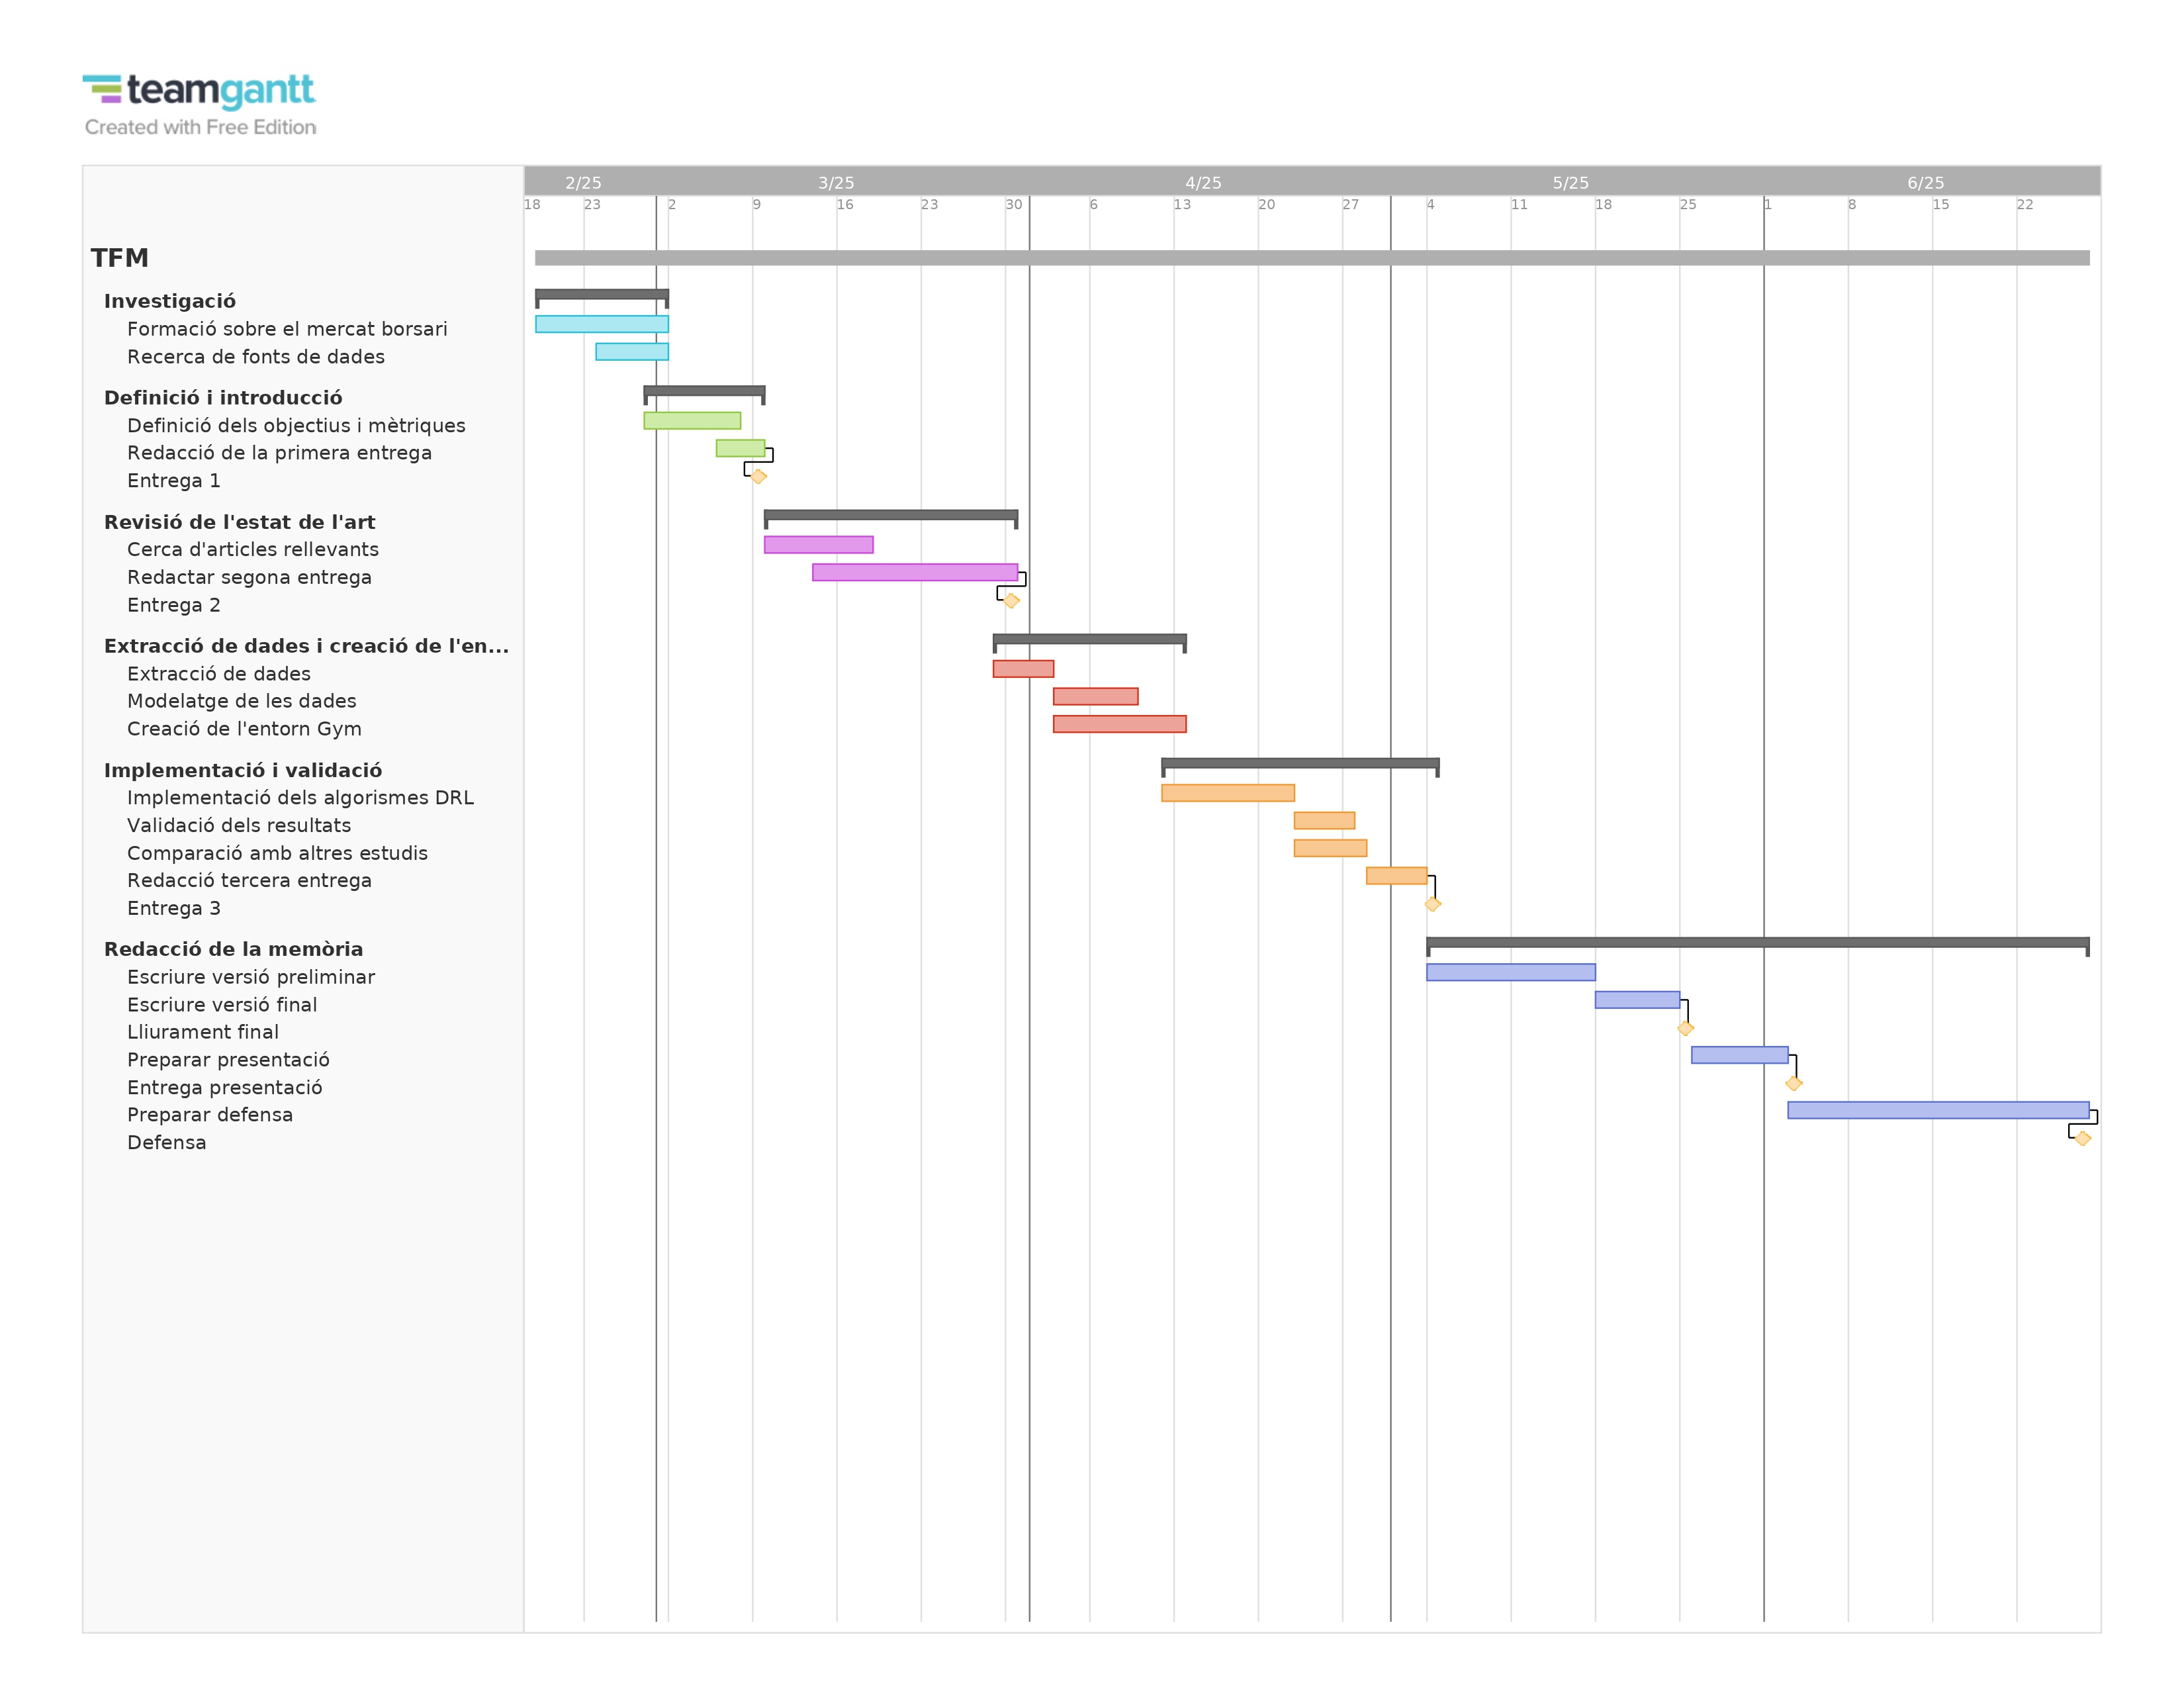
\includegraphics[width=1\textwidth]{figs/planning.jpg}
	\caption{Planificació del treball creada amb l'eina TeamGantt\cite{TeamGantt}.}
	\label{fig:context-anoni1}
\end{figure}


\subsection{Resum dels productes del projecte}

Els resultats d’aquest projecte inclouran el desenvolupament d’un agent d’inversió basat en Aprenentatge per Reforç Profund capaç d’integrar dades financeres i notícies processades mitjançant tècniques de NLP com TF-IDF, topic modeling (LDA) i anàlisi de sentiments. L’agent s’entrenarà en un entorn de simulació desenvolupat amb OpenAI Gym, on podrà analitzar dades de mercat i informació qualitativa per optimitzar la seva presa de decisions.

A més, es crearà una pipeline de processament de notícies per obtenir, netejar i transformar titulars de mitjans com The Guardian i The New York Times en una representació numèrica adequada per al model. Finalment, es durà a terme una avaluació detallada dels algorismes DQN, PPO i SAC mitjançant mètriques financeres com el Sharpe Ratio, Drawdown i retorn esperat, amb l’objectiu d’analitzar l’impacte de la integració de notícies en la presa de decisions.

% \subsection{Breu descripció de la resta de capítols de l'informe.}
% TBD

\chapter{Estat de l'art}

En aquest capítol s'exposen els fonaments teòrics i els treballs previs relacionats amb el desenvolupament d'agents d'inversió basats en Aprenentatge per Reforç Profund aplicats als mercats financers. Primerament, es revisa el concepte de trading i l'evolució cap al trading algorísmic per comprendre d'on sorgeix la necessitat d'aquestes noves estrategies. A continuació, es presenten els principis bàsics del DRL, juntament amb els algoritmes específics (Deep Q-Network, Proximal Policy Optimization i Soft Actor-Critic) que s'utilitzaran en aquest projecte.

A més, s'aborda la integració de dades qualitatives, com són en aquest cas les notícies, en els sistemes de decisió. També s'hi descriuen les principals tècniques de Processament del Llenguatge Natural que s'aplicaran en aquest treball. Finalment, es fa un repàs dels estudis i iniciatives que combinen DRL i NLP en l'àmbit financer.

\subsection{Introducció al trading}
\sloppy

Els mercats financers són un dels motors principals de l'economia global, ja que permeten la compra i venda d'actius com ara accions, bons, productes derivats o divises \cite{InvestopediaFinance}. Aquesta activitat permet a empreses i governs obtenir finançament, mentre que els inversors poden buscar rendiments ajustats al risc. Històricament, la presa de decisions en aquests mercats es basava en l'anàlisi fonamental, que se centra en l'estudi de factors macroeconòmics i de la situació financera de les empreses, i en l'anàlisi tècnic, que examina patrons de preu i volum al llarg del temps \cite{TradersBook}.

Amb l'evolució de la computació i la disponibilitat de bases de dades massives, les eines estadístiques i de machine learning han adquirit un pes rellevant en aquest àmbit. Això ha propiciat l'aparició del trading algorísmic, que consisteix en la implementació d'estratègies de compra i venda mitjançant algoritmes automàtics. 

Actualment, el trading el duen a terme tant inversors institucionals, com ara bancs d'inversió o fons d'alt risc, com inversors minoristes que accedeixen a plataformes en línia. Tot i que els objectius i les estratègies poden variar (des d'operacions de molt curt termini fins a enfocaments més orientats a llarg termini), l'element comú és la cerca del màxim retorn possible dins uns paràmetres de risc coneguts. En aquest context, l'aprenentatge automàtic i, de forma més recent, l'aprenentatge per reforç profund han sorgit com a eines per crear agents capaços d'adaptar-se a l'evolució dels mercats i maximitzar els resultats de les inversions.


\subsubsection{Tipus d'actius financers}
En els mercats financers, la unitat bàsica de transacció és l'actiu financer, un instrument que representa un valor econòmic i que pot ser comprat o venut sota determinades condicions. A grans trets, es poden agrupar en diverses categories segons el perfil de risc, la rendibilitat potencial o la seva naturalesa \cite{TypesOfInv}:

\begin{itemize}
    \item \textbf{Accions}: representen una part del capital social d'una empresa. El seu preu depèn de la demanda i l'oferta de mercat, així com de la salut financera i les expectatives de creixement de la companyia. Tenen una volatilitat alta, el que es tradueix en que poden aportar alts rendiments però el seu risc també és elevat.

    \item \textbf{Bons}: és deute emès per governs o empreses, que prometen un pagament periòdic d'interessos i la devolució del principal quan finalitzi un termini. Tot i que acostumen a tenir menys volatilitat que les accions, el seu preu també pot fluctuar segons factors macroeconòmics, tipus d'interès i risc d'impagament.

    \item \textbf{Matèries primeres i divises}: inclouen petroli, or, grans o altres productes, a més de monedes que s'intercanvien en mercats internacionals (FOREX). Els preus poden estar subjectes a factors geopolítics, condicions climàtiques o polítiques monetàries.

    \item \textbf{Fons i ETFs}: permeten invertir de manera diversificada en un conjunt d'actius dins una mateixa estructura (per exemple, un índex, un sector específic o un mercat geogràfic).
\end{itemize}

\subsubsection{Indicadors tècnics}
Els indicadors tècnics són equacions matemàtiques que fan servir el preu i, opcionalment, el volum d'un actiu per proporcionar informació que ajudi a identificar tendències i possibles punts de compra o venda de l'actiu. A continuació, es presenten els principals indicadors tècnics que s'apliquen en aquest projecte.

\paragraph{Mitjana mòbil simple (SMA)}
La mitjana mòbil simple (Simple Moving Average, SMA) és la mitjana aritmètica del preu de tancament (o d'un altre valor rellevant) en una finestra de temps $n$:

\begin{equation}
    \text{SMA}(t) = \frac{1}{n} \sum_{i=0}^{n-1} p_{t-i},
\end{equation}

on $p_{t-i}$ és el preu de tancament en l'instant $t-i$, i $n$ és la mida de la finestra. Les SMAs ajuden a suavitzar el soroll del preu i a detectar tendències de mitjà o llarg termini \cite{InvestopediaSMA}.

\paragraph{Índex de Força Relativa (RSI)}
L'índex de Força Relativa (RSI, Relative Strength Index) mesura la velocitat i el canvi en el moviment del preu, i pren valors entre 0 i 100. Es defineix a partir d'una mitjana de guanys i pèrdues en una finestra temporal (sovint 14 períodes). Una fórmula estàndard per calcular-lo és:

\begin{equation}
    \text{RS} = \frac{\text{Mitjana de guanys}}{\text{Mitjana de pèrdues}}
\end{equation}
\begin{equation}
    \text{RSI} = 100 - \left( \frac{100}{1 + \text{RS}} \right).
\end{equation}

Quan l'RSI supera un llindar, per exemple 70, s'entén que l'actiu podria estar en situació de sobrecompra, mentre que si se situa per sota de 30, pot indicar sobrevenda \cite{InvestopediaRSI}.

\paragraph{Moving Average Convergence Divergence (MACD)}
El MACD (Moving Average Convergence Divergence) és un indicador de tendència que es basa en la diferència entre dues mitjanes mòbils exponencials (EMA) de períodes diferents \cite{InvestopediaMACD}. Se'n fan servir dues: una ràpida (12 períodes) i una de lenta (26 períodes). La línia MACD es calcula com:

\begin{equation}
    \text{MACD}(t) = \text{EMA}_{\text{ràpida}}(t) - \text{EMA}_{\text{lenta}}(t),
\end{equation}

mentre que la línia senyal (signal line) sol ser una EMA de 9 períodes de la MACD:

\begin{equation}
    \text{Signal}(t) = \text{EMA}_{9}(\text{MACD}(t)).
\end{equation}

Si la línia MACD creua la línia senyal de baix a dalt, pot ser un senyal d'entrada alcista, i si la creua de dalt a baix sol indicar sortida o moviment baixista.

\begin{figure}[H]
	\centering
	\includegraphics[width=0.8\textwidth]{figs/macd.jpg}
	\caption{Histograma d'accions on s'observa el MACD i la senyal \cite{InvestopediaMACD}.}
	\label{fig:context-anoni1}
\end{figure}

\subsubsection{Trading algorísmic}
El trading algorísmic consisteix en l'execució d'ordres de compra i venda mitjançant algoritmes, habitualment sense requerir la intervenció d'un operador humà. Inicialment, aquests sistemes es van dissenyar per minimitzar el temps d'execució de les ordres, però amb els anys han evolucionat fins a incloure estratègies  basades en aprenentatge automàtic i aprenentatge profund\cite{Origins}.

El DRL ha donat lloc a agents capaços d'aprendre directament de la interacció amb el mercat. Aquests agents poden processar grans volums de dades i trobar correlacions poc evidents. Tanmateix, s'ha comprovat que la incorporació de dades complementàries, com les notícies, l'anàlisi de sentiments o les variables macroeconòmiques, pot millorar la robustesa i la precisió dels models \cite{DBLP}.



\subsection{Aprenentatge per reforç profund}

El DRL combina els principis de l'aprenentatge per reforç tradicional amb la potència de representació de les xarxes neuronals profundes. L'objectiu general és dissenyar un agent que interactua amb un entorn, prenent accions i obtenint una política òptima per maximitzar el retorn acumulat.


\begin{figure}[H]
	\centering
	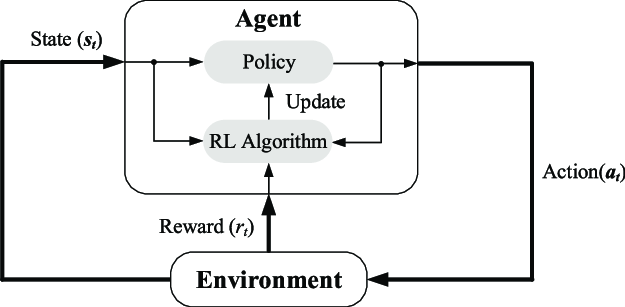
\includegraphics[width=0.8\textwidth]{figs/esquemaRL.png}
	\caption{Esquema d'interacció en el DRL\cite{esquemaRL}.}
	\label{fig:context-anoni1}
\end{figure}


Matemàticament, aquest problema es pot descriure mitjançant un procés de decisió de Markov, definit per $\langle \mathcal{S}, \mathcal{A}, p, r, \gamma\rangle$ \cite{DRLIntro}. El conjunt $\mathcal{S}$ representa els \emph{estats} possibles de l'entorn; $\mathcal{A}$ és el conjunt d'accions disponibles; $p(s' \mid s,a)$ és la probabilitat de transitar a l'estat $s'$ en executar l'acció $a$ a l'estat $s$; $r(s,a)$ defineix la recompensa obtinguda i $\gamma \in [0,1]$ és el factor de descompte que pondera les recompenses futures. A cada pas de temps $t$, l'agent observa un estat $s_t$, tria una acció $a_t$ i rep una recompensa $r_t$. L'objectiu final és maximitzar la suma de recompenses futures (retorn), expressada sovint com \cite{RLIntro}:

\begin{equation}
G_t \;=\; \sum_{k=0}^{\infty} \,\gamma^k \, r_{t+k+1}.
\end{equation}

\paragraph{Actors principals: agent, entorn, estat i acció}

\begin{itemize}
\item \textbf{Agent}: És el sistema que pren decisions a cada pas. L'agent manté o aprèn una estratègia, anomenada \emph{política} $\pi(a \mid s)$, que determina amb quina probabilitat triarà cada acció $a$ si es troba a l'estat $s$ \cite{M1}.

\item \textbf{Entorn}: És el medi extern on l'agent actua. Rep l'acció de l'agent i actualitza l'estat, retornant la nova observació $s_{t+1}$ i la recompensa $r_{t+1}$. L'entorn pot ser complex i contenir característiques molt variades, incloses dades numèriques i dades qualitatives provinents de fonts no estructurades, com poden ser les notícies \cite{M1}.

\item \textbf{Estat} ($s \in \mathcal{S}$): La informació rellevant del medi en un instant concret. Quan és tracta d'un sistema de Markov, es considera que $s$ conté tota la informació necessària per decidir l'acció òptima, sense haver de dependre de tots els estats previs \cite{M1}.

\item \textbf{Acció} ($a \in \mathcal{A}$): La decisió que pren l'agent en un estat determinat, com ara “comprar”, “vendre” o “mantenir” en un mercat financer \cite{M1}.
\end{itemize}

\paragraph{Funcions de valor i política}

En aprenentatge per reforç, l'agent aprèn funcions de valor per estimar la qualitat dels estats o de les accions. La funció de valor d'estat, $V^\pi(s)$, mesura el retorn esperat en trobar-se a l'estat $s$ i seguir la política $\pi$. De manera anàloga, la funció de valor d'acció, $Q^\pi(s,a)$, mesura el retorn esperat de prendre l'acció $a$ a l'estat $s$ i continuar amb la política $\pi$. Formalment \cite{M1}:

\begin{equation}
V^\pi(s) \;=\; \mathbb{E}_\pi\bigl[G_t \,\big\vert\, s_t = s\bigr]
\end{equation}
\begin{equation}
Q^\pi(s,a) \;=\; \mathbb{E}_\pi\bigl[G_t \,\big\vert\, s_t = s,\; a_t = a\bigr].
\end{equation}

La \textbf{política} òptima $\pi^*$ és aquella que maximitza el retorn acumulat; sovint, però, s'aprèn mitjançant aproximacions successives fins a trobar un bon resultat. Quan els espais d'estats o d'accions són molt grans, s'utilitzsen xarxes neuronals profundes per aproximar $Q$ o $V$ de manera eficient \cite{MnihNature2015}.

\vspace{2ex}
Dins d'aquest marc general, en el DRL s'han proposat diversos mètodes que resolen el problema de presa de decisions sota diferents estratègies de modelatge i optimització. A continuació, es descriuen els tres mètodes que s'han considerat en aquest treball.

\subsubsection{Deep Q-Network (DQN)}

El mètode Deep Q-Network (DQN) és un dels pilars fonamentals de l'aprenentatge per reforç profund (DRL), i representa l'aplicació directa de xarxes neuronals profundes per aproximar la funció d'acció-valor $Q(s, a)$ pròpia del mètode Q-learning. La seva introducció per DeepMind \cite{MnihNature2015} va marcar un abans i un després, aconseguint un rendiment superhumà en diversos jocs d'Atari.

\paragraph{Q-learning revisat:}


El mètode Q-learning és un algorisme de control de tipus off-policy que permet aprendre una política òptima mitjançant la maximització del valor esperat del retorn acumulat. La funció de valor $Q$ s’actualitza iterativament a partir de l’experiència de l’agent, segons la següent equació:

\begin{equation}
Q(s_t, a_t) \leftarrow Q(s_t, a_t) + \alpha \left[ r_{t+1} + \gamma \max_{a'} Q(s_{t+1}, a') - Q(s_t, a_t) \right]
\end{equation}

En aquesta fórmula, $\alpha$ representa la taxa d’aprenentatge, $r_{t+1}$ és la recompensa obtinguda després de realitzar l’acció $a_t$ en l’estat $s_t$, i $\gamma$ és el factor de descompte que pondera les recompenses futures. L’objectiu és ajustar progressivament l’estimació de $Q(s,a)$ per tal que reflecteixi millor els guanys a llarg termini que pot aconseguir l’agent en seguir una política determinada.

\paragraph{Limitacions i solució amb DQN:}

Tot i la seva simplicitat conceptual, Q-learning presenta limitacions importants quan s’aplica a problemes amb espais d’estats molt grans o continus. En aquests casos, la representació explícita de la taula $Q(s,a)$ no es pot executar, tant per qüestions de memòria com per l'eficiència computacional. Per abordar aquest problema, es va proposar l’algorisme Deep Q-Network (DQN), que substitueix la taula Q per una xarxa neuronal capaç d’aproximar la funció $Q(s,a)$ a través de paràmetres ajustables $\theta$, de manera que $Q(s,a; \theta) \approx Q^*(s,a)$.


\paragraph{Arquitectura DQN:}

L’arquitectura d’una DQN es basa habitualment en una xarxa neuronal profunda, que pot adaptar-se segons la naturalesa de les dades d’entrada. Per exemple, si es treballa amb imatges, s’utilitzen xarxes convolucionals (CNN), mentre que en altres casos es poden fer servir xarxes totalment connectades o altres estructures. El resultat de la xarxa és un vector que conté els valors Q estimats per a cada acció possible a partir d’un estat donat.


\paragraph{Funció de pèrdua i entrenament:}
El procés d’aprenentatge es fonamenta en la minimització de la diferència entre la sortida de la xarxa i un valor objectiu $y_t$, que s’obté aplicant la fórmula de Bellman. La funció de pèrdua utilitzada habitualment és la següent:

\begin{equation}
\mathcal{L}(\theta) = \mathbb{E}_{(s,a,r,s') \sim \mathcal{D}} \left[ \left( y_t - Q(s, a; \theta) \right)^2 \right]
\end{equation}

on el valor objectiu es calcula com $y_t = r + \gamma \max_{a'} Q(s', a'; \theta^-)$, i $\theta^-$ representa els pesos d’una còpia fixa de la xarxa principal (target network) que s’actualitza periòdicament.


\paragraph{Tècniques per estabilitzar DQN:}
Per millorar el comportament i l’estabilitat del model durant l’entrenament, DQN incorpora diverses estratègies. En primer lloc, s’utilitza una target network, és a dir, una rèplica de la xarxa principal amb pesos congelats durant diverses iteracions, que permet calcular les prediccions de futur de manera més estable. En segon lloc, s’emprèn la tècnica d’experience replay, que consisteix a emmagatzemar les transicions observades $(s,a,r,s')$ en una memòria i mostrejar-les aleatòriament durant l’entrenament. Això trenca la correlació temporal entre mostres i millora l’eficiència de l’aprenentatge. Finalment, per garantir un equilibri entre exploració i explotació, s’adopta una política $\varepsilon$-greedy, en què l’agent selecciona accions aleatòries amb una probabilitat $\varepsilon$, afavorint l'exploració durant l'entrenament.

\begin{itemize}
  \item \textbf{Target network:} Una segona xarxa amb pesos fixos $\theta^-$ utilitzada per calcular els valors objectiu $y_t$ durant un cert nombre d'iteracions.
  \item \textbf{Experience replay:} S'emmagatzemen les transicions $(s,a,r,s')$ en una memòria (buffer), des d'on es mostregen de manera aleatòria per trencar correlacions temporals i millorar l'eficiència de l'entrenament.
  \item \textbf{$\varepsilon$-greedy:} Política exploratòria que escull accions aleatòries amb probabilitat $\varepsilon$, afavorint l'exploració durant l'entrenament.
\end{itemize}


\subsubsection{Proximal Policy Optimization (PPO)}

El mètode Proximal Policy Optimization (PPO) és un dels algorismes d'aprenentatge per reforç profund més utilitzats actualment. Va ser proposat per OpenAI com una alternativa robusta i eficient als mètodes de gradient de política tradicionals com REINFORCE o TRPO (Trust Region Policy Optimization)\cite{}. Es caracteritza per combinar estabilitat,  eficiència en el càlcul i ser fàcilment implementable.

\paragraph{Fonaments:}

Es tracta d'un mètode basat en gradient de política (Policy Gradient, PG). Aquests mètodes actualitzen els paràmetres de la política directament segons:

\begin{equation}
\theta_{t+1} \leftarrow \theta_t + \alpha \nabla_\theta J(\theta)
\end{equation}

on $J(\theta)$ és una estimació del retorn esperat. Tanmateix, actualitzacions massa grans poden trencar la política i provocar divergències. PPO simplifica aquesta idea limitant els canvis de política mitjançant una funció de pèrdua acotada.

\paragraph{Objectiu de PPO:}

PPO optimitza la política maximitzant l'objectiu següent, anomenat \textit{clipped surrogate objective}:

\begin{equation}
\mathcal{L}^{\text{CLIP}}(\theta) = \mathbb{E}_t \left[ \min \left( r_t(\theta) \hat{A}_t, \, \text{clip}(r_t(\theta), 1 - \epsilon, 1 + \epsilon) \hat{A}_t \right) \right]
\end{equation}

on:
\begin{itemize}
  \item $r_t(\theta) = \frac{\pi_\theta(a_t | s_t)}{\pi_{\theta_{\text{old}}}(a_t | s_t)}$ és el quocient de probabilitats entre la nova política i l'antiga.
  \item $\hat{A}_t$ és l'avantatge estimat en el temps $t$, usualment calculat com $\hat{A}_t = Q(s_t,a_t) - V(s_t)$.
  \item $\epsilon$ és un hiperparàmetre que controla l'amplitud del clip, típicament entre 0.1 i 0.3.
\end{itemize}

Aquesta formulació garanteix que si la nova política s'allunya massa de l'antiga ($r_t$ fora dels límits), l'actualització es trunca i no es premia, evitant grans desviacions.

\paragraph{Estimació de l'avantatge:}

Per reduir la variància en l'estimació de l'avantatge s'utilitza sovint el mètode \textbf{GAE (Generalized Advantage Estimation)}:

\begin{equation}
\hat{A}_t = \sum_{l=0}^{\infty} (\gamma \lambda)^l \delta_{t+l}
\end{equation}

on $\delta_t = r_t + \gamma V(s_{t+1}) - V(s_t)$ i $\lambda$ és un hiperparàmetre que controla el trade-off entre biaix i variància.

\paragraph{Algorisme complet:}

A cada iteració, PPO executa els següents passos:
\begin{enumerate}
  \item Recollida de trajectòries amb la política actual $\pi_\theta$.
  \item Càlcul del retorn, la funció de valor $V(s)$ i l'avantatge $\hat{A}_t$.
  \item Entrenament durant diverses èpoques minimitzant $\mathcal{L}^{\text{CLIP}}(\theta)$ amb optimitzadors com Adam.
  \item Actualització de la política antiga: $\theta_{\text{old}} \leftarrow \theta$.
\end{enumerate}


\subsubsection{Soft Actor-Critic (SAC)}

Soft Actor-Critic (SAC) és un dels algoritmes d'aprenentatge per reforç profund més eficients actualment, especialment adequat per a entorns continus. S'emmarca dins la classe dels mètodes \textit{actor-crític off-policy}, amb la novetat d'optimitzar no només el retorn esperat sinó també l'entropia de la política, afavorint polítiques més deterministes i exploratòries.

\paragraph{Entropia i motivació:}

En lloc de maximitzar només el retorn esperat acumulat, SAC maximitza l'objectiu següent:

\begin{equation}
J(\pi) = \mathbb{E}_{\tau \sim \pi} \left[ \sum_t r(s_t, a_t) + \alpha \mathcal{H}(\pi(\cdot|s_t)) \right]
\end{equation}

on $\mathcal{H}$ és l'entropia de la política, i $\alpha$ és un hiperparàmetre que pondera l'exploració. Aquest terme afavoreix polítiques que mantinguin accions aleatòries durant més temps, evitant una convergència massa ràpida.

\paragraph{Components del SAC:}

SAC combina tres xarxes neuronals clau:

\begin{itemize}
  \item \textbf{Actor} $\pi_\phi(a|s)$: Política estocàstica que genera accions a partir d'una distribució parametritzada (normalment gaussiana).
  \item \textbf{Crítics} $Q_{\theta_1}(s,a)$ i $Q_{\theta_2}(s,a)$: Dues funcions de valor d'acció per reduir el sobreaprenentatge mitjançant la minimització del valor més baix.
  \item \textbf{Target critics}: Versions retardades dels crítics per a una actualització estable.
\end{itemize}

\paragraph{Objectius d'entrenament:}

\begin{itemize}
  \item \textbf{Actualització dels crítics:} s'ajusten per minimitzar l'error TD sobre la següent estimació soft del retorn:

  \begin{equation}
  y(r,s') = r + \gamma \left( \min_{i=1,2} Q_{\theta'_i}(s', a') - \alpha \log \pi_\phi(a'|s') \right)
  \end{equation}

  \item \textbf{Actualització de l'actor:} es minimitza:

  \begin{equation}
  \mathcal{L}_{\text{actor}} = \mathbb{E}_{s_t \sim \mathcal{D}} \left[ \alpha \log \pi_\phi(a_t|s_t) - Q_{\theta}(s_t, a_t) \right]
  \end{equation}

  \item \textbf{Actualització de l'entropia:} es pot ajustar automàticament $\alpha$ mitjançant:

  \begin{equation}
  \mathcal{L}(\alpha) = \mathbb{E}_{a_t \sim \pi} \left[ -\alpha \log \pi(a_t|s_t) - \alpha \mathcal{H}_\text{target} \right]
  \end{equation}

\end{itemize}

\paragraph{Característiques clau:}

\begin{itemize}
  \item \textbf{Off-policy:} Fa ús de replay buffer, millorant l'eficiència de la mostra.
  \item \textbf{Exploració regularitzada:} L'entropia manté l'exploració activa durant l'entrenament.
  \item \textbf{Dues xarxes Q:} Redueixen el biaix en les estimacions de valor.
  \item \textbf{Entropia adaptable:} $\alpha$ pot ser un paràmetre aprés per ajustar el trade-off entre exploració i explotació.
\end{itemize}




\begin{table}[h]
\centering
\caption{Comparativa dels algoritmes de DRL utilitzats}
\begin{tabular}{lccc}
\hline
\textbf{Característica} & \textbf{DQN} & \textbf{PPO} & \textbf{SAC} \\ \hline
Tipus & Basat en valor & Basat en política & Actor-Crític \\
Espai d'accions & Discret & Discret/Continu & Continu \\
Exploració & $\epsilon$-greedy & Clipping gradient + GAE & Maximització entropia \\
Replay buffer & Sí & No & Sí \\
Estabilitat & Moderada & Alta & Alta \\ \hline
\end{tabular}
\label{tab:comparativa_algoritmes}
\end{table}



\subsection{Natural language processing}

 Les tècniques de Processament del Llenguatge Natural (NLP) permeten extreure característiques clau dels textos, ja sigui en forma de paraules rellevants, temàtiques predominants o sentiments. A continuació es descriuen les tècniques que s'han considerat en aquest treball.

\subsubsection{TF-IDF}

El \emph{Term Frequency–Inverse Document Frequency} (TF-IDF) és una mesura que valora la importància d'una paraula dins d'un document $d$, tot penalitzant les paraules que apareixen amb molta freqüència a la col·lecció global de textos o documents \cite{Ramos2003}. Està composta de dos factors:

\begin{itemize}
\item \textbf{Term Frequency (TF):} la freqüència relativa d'aparició del mot $t$ en el document $d$. Una definició habitual és:
\[
\mathrm{TF}(t,d) \;=\; \frac{f_{t,d}}{\sum_{t' \in d} f_{t',d}},
\]
on $f_{t,d}$ és el nombre d'aparicions de $t$ en $d$.
\item \textbf{Inverse Document Frequency (IDF):} penalitza les paraules molt comunes en el conjunt de textos. Una forma estàndard és:
\[
\mathrm{IDF}(t,D) \;=\; \ln \Bigl(\frac{|D|}{\,|\{\,d \in D : t \in d\,\}|}\Bigr),
\]
on $D$ és el conjunt de tots els documents.
\end{itemize}

La mesura TF-IDF final per a un mot $t$ en un document $d$ és el producte dels dos factors:
\[
\mathrm{TF\text{-}IDF}(t,d) \;=\; \mathrm{TF}(t,d)\;\cdot\;\mathrm{IDF}(t,D).
\]

En contextos financers, aquesta representació pot destacar termes específics que siguin indicatius d'esdeveniments rellevants (p. ex., \emph{crisi}, \emph{fusió}, \emph{banc central}) que poden anticipar canvis de mercat.

\subsubsection{Topic Modeling (LDA)}

El \emph{Topic Modeling} busca descobrir temàtiques latents en un conjunt de documents de manera no supervisada. Latent Dirichlet Allocation (LDA) és un dels models més populars \cite{Blei2003}. LDA assumeix que:

\begin{itemize}
\item Cada document és una barreja de temes en diferents proporcions.
\item Cada tema és una distribució de probabilitat sobre el vocabulari.
\end{itemize}

Formalment, si es tenen $K$ temes i $D$ documents, LDA estima distribucions $\theta_d$ (barreges de temes del document $d$) i $\phi_k$ (distribució de paraules del tema $k$). En aquest cas, un cop inferit, es pot assignar a cada notícia la probabilitat de pertànyer a cada tema, creant un vector de característiques que es pot incorporar a l'estat de l'agent.

\begin{figure}[H]
	\centering
	\includegraphics[width=0.8\textwidth]{figs/tm.png}
	\caption{Esquema del funcionament del Topic Modeling\cite{esquemaRL}.}
	\label{fig:context-anoni1}
\end{figure}

\subsubsection{Anàlisi de sentiments}

L'anàlisi de sentiments pretén determinar la polaritat (positiva, negativa o neutra) d'un text. Les tècniques més senzilles es basen en diccionaris de paraules amb connotació positiva o negativa, mentre que els mètodes avançats utilitzen models supervisats o xarxes neuronals de tipus \emph{Transformers}. En l'àmbit financer, detectar ràpidament un sentiment negatiu pot anticipar vendes massives, mentre que un sentiment marcadament positiu pot indicar expectatives alcistes del mercat.


\subsection{Integració de NLP i DRL}

La utilització de tècniques NLP en agents DRL s'ha convertit en una possible estratègia per al desenvolupament de sistemes de trading algorítmic més informats i adaptatius. Aquesta combinació permet incorporar no només dades numèriques històriques com preus o volums, sinó també informació qualitativa provinent de diferents fonts, com ara notícies financeres o xarxes socials.

Tot i que la literatura en aquest àmbit no és extensa, hi ha publicacions que tracten aquest tema. Per exemple, en \cite{gangopadhyay}, es proposa un model DDPG (Deep Deterministic Policy Gradient) enriquit amb embeddings semàntics de notícies per millorar les decisions d'inversió. Els resultats mostren una millora significativa en el rendiment de l'algoritme d'inversió.

En un altre estudi rellevant és un treball de final de grau, \cite{alvarez2023real}, on s'utilitzen representacions BERT de notícies financeres en temps real combinades amb informació de mercat per alimentar un agent DRL. Aquest sistema demostra una millor capacitat d'anticipació de tendències respecte a models que només utilitzen dades numèriques.

A més, s'ha observat que la incorporació d'informació provinent de xarxes socials, com Twitter o Reddit, pot afegir valor predictiu. En \cite{DBLP}, es mostra que els senyals socials poden millorar l'eficiència d'agents basats en DQN i PPO quan s'apliquen a mercats volàtils com el de les criptomonedes.





% \chapter{Glossari}
% Definició dels termes y acrònims més rellevants utilitzats en aquest informe.
% \begin{itemize}
%     \item API (Application Programming Interface): interfície que especifica com diferents components de programes informàtics poden interactuar.
%     \item Drawdown: Mesura financera que representa la pèrdua màxima des d'un pic fins a un mínim abans d’una recuperació en el rendiment d'una inversió.
%     \item DQN (Deep Q-Network): Algorisme de DRL que utilitza xarxes neuronals per aproximar la funció de valor Q.
%     \item DRL (Deep Reinforcement Learning): Aprenentatge per reforç profund, una branca del Machine Learning que combina l’Aprenentatge per Reforç (RL) amb xarxes neuronals profundes.
%     \item Gym (OpenAI Gym): Entorn de simulació utilitzat per al desenvolupament i avaluació d'algoritmes d'Aprenentatge per Reforç. 
%     \item LDA (Latent Dirichlet Allocation): Model probabilístic de generació de temes utilitzat en NLP per trobar termes equivalents.
%     \item NLP (Natural Language Processing): Camp de la Intel·ligència Artificial que estudia la interacció entre ordinadors i llenguatge humà.
%     \item PPO (Proximal Policy Optimization): Algorisme de DRL que optimitza les polítiques d'acció amb estabilitat i eficiència
%     \item SAC (Soft Actor-Critic): Algorisme de DRL que utilitza aprenentatge basat en entropia per millorar la presa de decisions en entorns continus.
%     \item TF-IDF (Term Frequency-Inverse Document Frequency): Tècnica de NLP utilitzada per avaluar la importància d'una paraula en un document dins d'un conjunt de documents.
    
% \end{itemize}



% bibliografía
\addcontentsline{toc}{chapter}{Bibliografía}
\bibliographystyle{plain}
\bibliography{referencias}

\end{document}
